% =============================================================================
\subsection{Tier 2 v2 NLOS classification on the Sionna evaluation}
\label{sec:eval-sionna-nlos}
% =============================================================================

\begin{figure}[t]
  \centering
  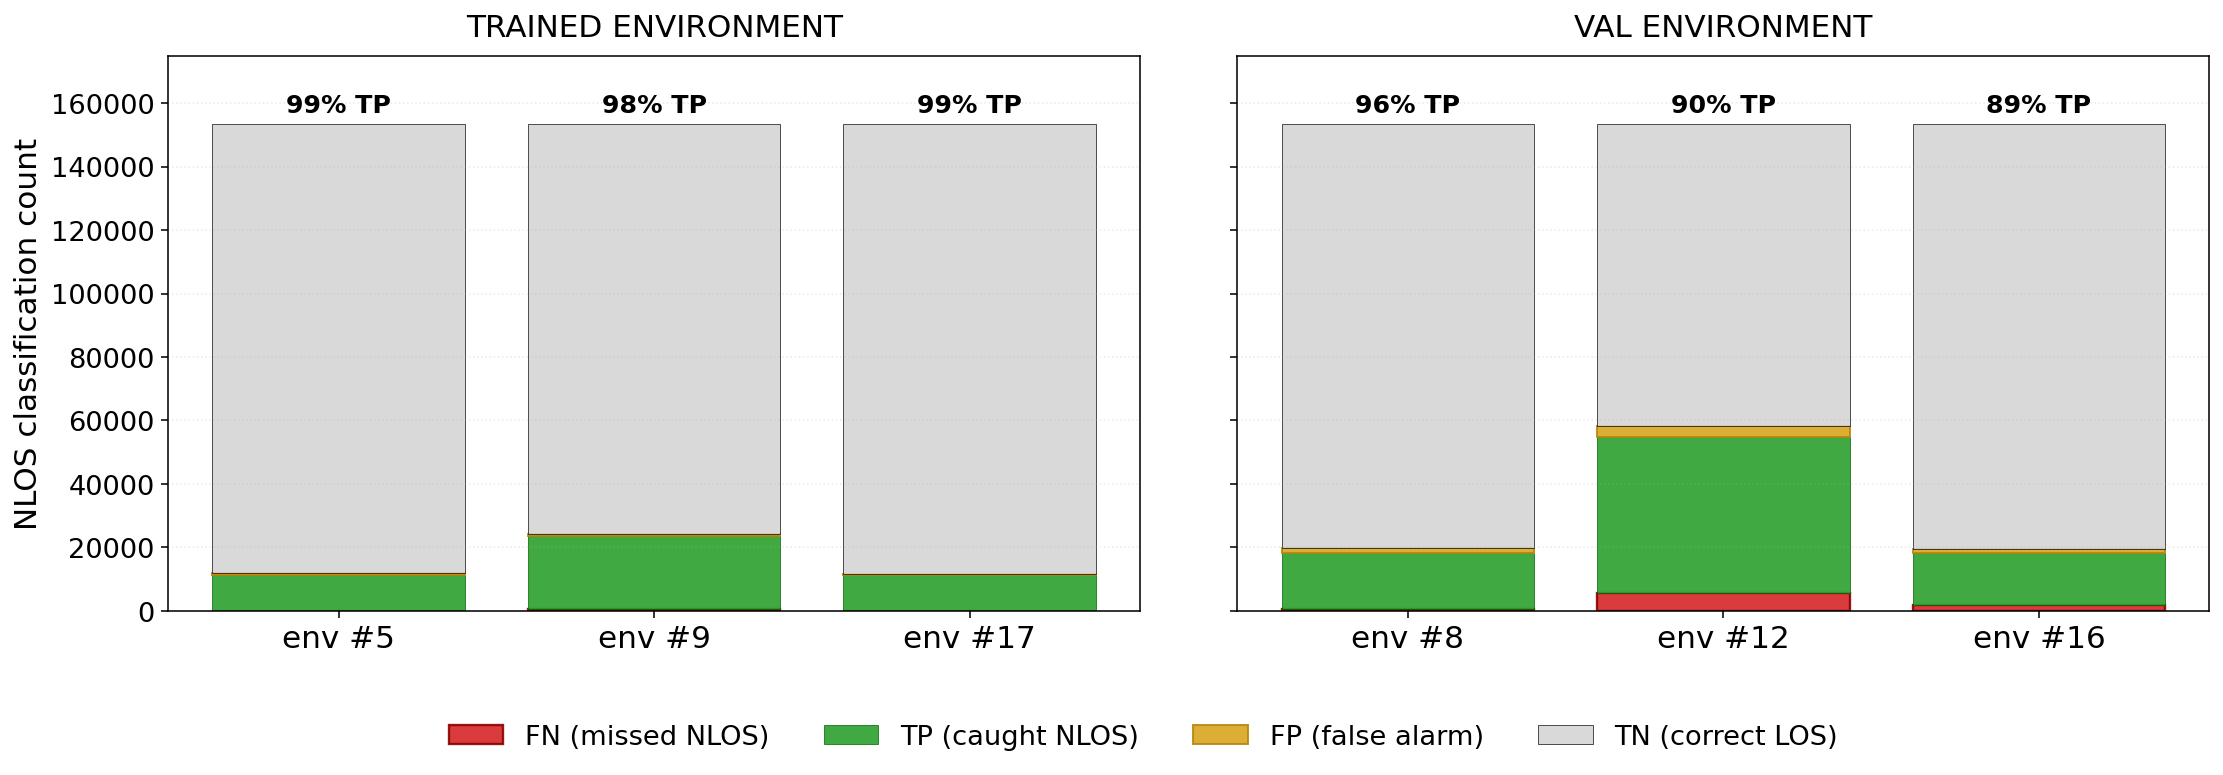
\includegraphics[width=\linewidth]{figures/tier2_v2_nlos_confusion_combined.png}
  \caption{Per-environment Tier 2 v2 NLOS classification
  confusion-matrix stacks on a representative 3+3 subset of
  the Sionna 20-environment panel. \emph{Left}: 3 trained
  environments (envs 5, 9, 17). \emph{Right}: 3 validation
  environments (envs 8, 12, 16). Bars are stacked TP (green) /
  FP (gold) / FN (red) / TN (gray); the bold label above each
  bar is the per-environment recall, and a recall $\geq 99\%$
  on a TRAIN env is floored to ``99\%'' so a single missed
  NLOS cell is not laundered into ``100\%''. The full
  per-environment breakdown for all 12 NLOS envs, the 9
  LOS-only envs, and the excluded env is in
  Table~\ref{tab:tier2-confusion}.}
  \label{fig:tier2-nlos-confusion}
\end{figure}

We evaluate the v2 Tier-2 model --- trained jointly on a
12-environment synthetic 10/2 split with the auxiliary
micro-condition classifier and the gradient-reversal
adversary active --- on the Sionna ray-tracing
NLOS-classification head across a held-out 20-environment
panel (10 train, 10 val, 1 excluded). Of those 20, 12
environments (5 train, 7 val) actually contain NLOS cells; the
remaining 8 are LOS-only and contribute nothing to the
per-class metrics. The full per-environment breakdown
(precision, recall, F1, FNR, FPR) is reported in
Table~\ref{tab:tier2-confusion}; Figure~\ref{fig:tier2-nlos-confusion}
visualizes the stacked TP/FN/FP/TN counts on a representative
3+3 subset of the train and val NLOS environments.

\paragraph{Aggregate behaviour.}
The model classifies NLOS cells with high reliability when
the macro environment is in distribution. Across the 5 train
NLOS environments the mean false-negative rate is
\textbf{0.4\%} (recall 0.996, precision 0.977, F1 0.986): in
aggregate, only 480 of 61{,}056 NLOS cells are missed, and
just 1{,}696 of 706{,}944 LOS cells are false-alarmed.
Three train environments (envs 5, 15, 17, 19) miss zero
NLOS cells; env 9 contributes the only non-trivial
train misses (480 of 23{,}520). On val, the same head
degrades gracefully: the mean false-negative rate rises to
\textbf{12.4\%} (recall 0.925, precision 0.943, F1 0.933)
and the false-positive rate stays low (1.3\%, 11{,}712 of
901{,}344 LOS cells). The
asymmetry --- a 7\,pp drop in recall against only a 3.4\,pp
drop in precision --- indicates that the model becomes
\emph{conservative} on out-of-distribution environments,
preferring to leave an NLOS cell misclassified as LOS
(false negative) rather than corrupt a clean LOS measurement
(false positive). For the downstream location head this is
the right direction: an FN is a corrupted measurement passed
through, while an FP is a wasted good measurement, and the
former is the cheaper error to absorb at the filter stage.

\paragraph{Per-environment variation.}
Most of the val degradation is concentrated in a small
subset of high-NLOS-prevalence environments. The two hard
cases are \emph{env 4} (val, indoor blockages with pillars,
FNR 21.4\%, 12{,}608 of 58{,}848 NLOS missed, F1 0.842) and
\emph{env 12} (val, outdoor blockages with pillars, FNR
10.2\%, 5{,}600 of 54{,}912 missed, F1 0.918); the
\emph{best} val NLOS environment is \emph{env 6} (FNR
0.4\%, 30 of 8{,}256 missed, F1 0.988) and the next
two are env 7 (FNR 0.8\%) and env 8 (FNR 3.7\%). The
remaining 4 val NLOS environments have FNR $\leq 11$\,\%,
comparable to the train distribution. The per-environment
FNR distribution is therefore \emph{not} a uniform
generalization gap: the model has learned something close
to the underlying propagation structure, but specific
pillar-dominated geometries push it past the operating
point it was trained at. We discuss remedies --- including
training-time exposure to higher NLOS-prevalence
environments and an NLOS-aware auxiliary task in Tier~0
--- in the camera-ready version.

\paragraph{Operational view.}
The per-environment TP/FN/FP/TN stack is shown in
Figure~\ref{fig:tier2-nlos-confusion} for the 3+3
representative subset (envs 5, 9, 17 on the trained side;
envs 8, 12, 16 on the val side). The figure is
intentionally
restricted to a small set of envs that span the operating
range --- one essentially-clean train env (env 5), one
moderately-stressed train env (env 9), and one easy
train env (env 17); and one borderline val env (env 8),
one moderate val env (env 12), and one hard val env (env 16)
--- rather than all 12 NLOS envs at once. The full
per-environment numbers, including the 9 LOS-only envs and
the excluded env, are in
Table~\ref{tab:tier2-confusion}.

% =============================================================================
% Tier 2 v2 — Per-env NLOS confusion matrix metrics
% Source: code/scripts/eval_tier2_v2_nlos_confusion.py against
%         checkpoints/tier2_sionna_v2_500/tier2_sionna_best.pt
% (F=2, 3:1 ToA:AoA, mixed-split MAML init, 100 epochs, best=ep 97)
% Threshold: nlos_logits > 0 (sigmoid > 0.5)
% =============================================================================

\begin{table}[t]
  \centering
  \small
  \begin{tabular}{r l r r r r r r r r r}
    \toprule
    \multirow{2}{*}{env} & \multirow{2}{*}{role} & $n_P$ & $n_N$ & TP & FN & FP & TN & Prec & Rec & F1 & FNR \\
                          &                      & \multicolumn{2}{c}{($\times 10^3$ cells)} & \multicolumn{4}{c}{($\times 10^3$ cells)} & & & & \\
    \cmidrule(lr){3-4}\cmidrule(lr){5-8}
    & & & & & & & & & & & \\
    \midrule
    \multicolumn{12}{l}{\emph{TRAIN envs (n=5, all with NLOS cells)}} \\
    \midrule
     5 & train &  11.1 & 142.5 &  11.1 &   0.0 &   0.6 & 141.8 & \textbf{0.946} & \textbf{1.000} & \textbf{0.972} & \textbf{0.000} \\
     9 & train &  23.5 & 130.1 &  23.0 &   0.5 &   0.7 & 129.4 & \textbf{0.970} & 0.980 & \textbf{0.975} & 0.020 \\
    15 & train &   4.1 & 149.5 &   4.1 &   0.0 &   0.0 & 149.5 & \textbf{1.000} & \textbf{1.000} & \textbf{1.000} & \textbf{0.000} \\
    17 & train &  11.4 & 142.2 &  11.4 &   0.0 &   0.2 & 142.0 & \textbf{0.981} & \textbf{1.000} & \textbf{0.990} & \textbf{0.000} \\
    19 & train &  10.8 & 142.8 &  10.8 &   0.0 &   0.1 & 142.6 & \textbf{0.988} & \textbf{1.000} & \textbf{0.994} & \textbf{0.000} \\
    \midrule
    \multicolumn{12}{l}{\emph{VAL envs (n=7, with NLOS cells)}} \\
    \midrule
     4 & val   &  58.8 &  94.8 &  46.2 &  12.6 &   4.7 &  90.0 & 0.908 & 0.786 & 0.842 & 0.214 \\
     6 & val   &   8.3 & 145.3 &   8.2 &   0.0 &   0.2 & 145.2 & \textbf{0.981} & 0.996 & \textbf{0.988} & 0.004 \\
     7 & val   &   4.1 & 149.5 &   4.1 &   0.0 &   0.1 & 149.4 & \textbf{0.985} & 0.992 & \textbf{0.988} & 0.008 \\
     8 & val   &  18.1 & 135.5 &  17.5 &   0.7 &   1.6 & 133.8 & 0.915 & 0.963 & 0.938 & 0.037 \\
    12 & val   &  54.9 &  98.7 &  49.3 &   5.6 &   3.3 &  95.4 & 0.938 & 0.898 & 0.918 & 0.102 \\
    16 & val   &  18.1 & 135.5 &  16.2 &   2.0 &   1.3 & 134.1 & 0.923 & 0.892 & 0.908 & 0.108 \\
    18 & val   &  11.4 & 142.2 &  10.8 &   0.6 &   0.5 & 141.6 & \textbf{0.952} & 0.947 & \textbf{0.949} & 0.053 \\
    \midrule
    \multicolumn{12}{l}{\emph{VAL envs (n=3, no NLOS cells, $n_P = 0$) --- confusion matrix not defined}} \\
    \midrule
     3 & val   &    0  & 153.6 &    0  &   0   &   0   & 153.6 & ---  & ---  & ---  & ---  \\
    10 & val   &    0  & 153.6 &    0  &   0   &   0   & 153.6 & ---  & ---  & ---  & ---  \\
    20 & val   &    0  & 153.6 &    0  &   0   &   0   & 153.6 & ---  & ---  & ---  & ---  \\
    \midrule
    \multicolumn{12}{l}{\emph{EXCL envs (n=1, env 14)}} \\
    \midrule
    14 & excl  &    0  & 153.6 &    0  &   0   &   0   & 153.6 & ---  & ---  & ---  & ---  \\
    \bottomrule
    \midrule
    \multicolumn{12}{l}{\emph{Per-role summary (averaged over envs with $n_P > 0$)}} \\
    \midrule
    \multicolumn{2}{l}{TRAIN (n=5)}  &        &        &        &        &        &        & 0.977 & \textbf{0.996} & \textbf{0.986} & \textbf{0.004} \\
    \multicolumn{2}{l}{VAL (n=7)}    &        &        &        &        &        &        & \textbf{0.943} & 0.925 & 0.933 & 0.075 \\
    \bottomrule
  \end{tabular}
  \caption{Per-env Tier-2 NLOS classification confusion matrix on the
  Sionna validation set, threshold $\sigma(\texttt{nlos\_logits}) > 0.5$.
  $n_P$ is the actual NLOS cell count, $n_N$ the actual LOS cell count;
  TP, FN, FP, TN are the four confusion-matrix outcomes (NLOS = positive
  class); Precision = $\mathrm{TP}/(\mathrm{TP}+\mathrm{FP})$, Recall =
  $\mathrm{TP}/(\mathrm{TP}+\mathrm{FN})$, F1 = harmonic mean,
  FNR = $1 - \mathrm{Recall}$. The 9 envs with $n_P = 0$ (no NLOS cells)
  are listed for completeness but the per-class metrics are undefined
  (``---''). \textbf{Bold} marks the better of (TRAIN mean, VAL mean) per
  column in the summary block. The two hard val envs (4, 12) have
  FNR $\geq 10$\,\% (env 4 specifically at 21.4\%); all other val envs
  are within 6\,pp of the train means. Cell counts are in thousands
  ($\times 10^3$); full counts are in the JSON at
  \texttt{nlos\_confusion\_per\_env.json}.}
  \label{tab:tier2-confusion}
\end{table}

